\subsection{Cenários energéticos e a matriz elétrica brasileira}
\begin{onehalfspace}
    O cenário energético mundial vem apresentando progressos quanto ao desenvolvimento da 
    eficiência energética e da busca de fontes limpas e renováveis de energia. A criação de 
    políticas de redução de consumo energético, assim como a promoção de congressos, eventos 
    e demais incentivos à pesquisa e desenvolvimento acadêmico apontam melhorias neste âmbito 
    da energia \cite{InternationalEnergyAgency-IEA2014}.\newline
    Estudo desenvolvido pela \textcite{UnitedNations2017} aponta que 103 países definiram 
    a eficiência energética e uso de energias renováveis como parte importante do seu 
    planejamento estratégico, e destes, 79 são países emergentes e em desenvolvimento. 
    Constata-se, ainda, que o consumo de energia poderia ter sido 12\% maior em 2017 caso as 
    políticas públicas mencionadas anteriormente não tivessem sido implementadas desde o ano 
    2000 \cite{InternationalEnergyAgency-IEA2019b}.\newline
    Entre os países emergentes e em desenvolvimento, nota-se que há um esforço para redução 
    de consumo de energia, o que reflete em fatores como o aumento da segurança energética, 
    aumento na competitividade industrial, redução de emissão de poluentes e da degradação 
    ambiental, expansão ao acesso de energia, além da indução ao crescimento econômico 
    \cite{BancoMundial2018}. Entretanto, de acordo com \textcite{Abramovay2010,Abramovay2014}, 
    a matriz energética mundial ainda será predominantemente composta por fontes fósseis de 
    energia até meados do século XXI.\newline
    No Brasil, a taxa de consumo energético, assim como em outros países, é definida pelo 
    aquecimento econômico e cenários estabelecidos para o desenvolvimento esperado para o país. 
    Nesse sentido, espera-se que o Brasil, até 2026, apresente crescimento econômico e, 
    concomitantemente, consuma energia de forma modesta. Projeta-se que este crescimento seja 
    da ordem de 1,9\% ao ano até a metade da década analisada, com variações que definem o 
    crescimento do consumo em 2,3\% anuais, indicando otimismo para o setor de energia 
    brasileiro \cite{EmpresadePesquisaEnergetica-EPE2017,EmpresadePesquisaEnergetica-EPE2017a}.\newline
    Em 2018, a geração hídrica respondeu por 66,6\% da oferta interna entre as fontes de 
    produção de energia elétrica no Brasil, seguido do gás natural, com 8,6\%, da biomassa, 
    com 8,5\% e de outras fontes, 16,3\%, como mostrado no Gráfico \ref{Grafico 1}. Deste modo, 
    as centrais hidráulicas de serviço público e de autoprodução contribuíram para expansão 
    da capacidade total instalada de geração de energia elétrica, com acréscimo de 3.864 MW 
    dos 5.728 MW, ou 67,5\% do total adicionado \cite{EmpresadePesquisaEnergetica-EPE2019}.
    \begin{figure}[h]
        \centering
        \caption{\small Oferta interna de energia elétrica no Brasil (a) e a participação setorial de consumo de eletricidade (b).}
        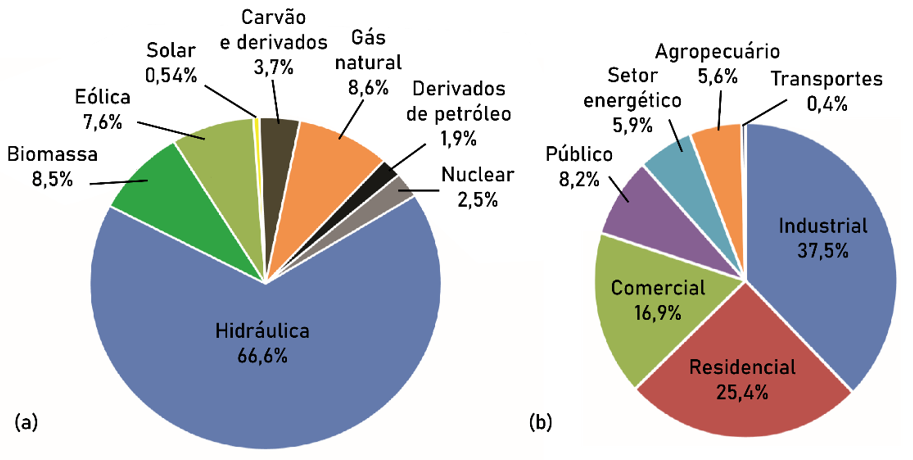
\includegraphics[width=0.8\textwidth]{graphs/graph1.png}
        %\small Fonte: adaptado de Kurnitski et al. (2011, tradução nossa)
        \label{Grafico 1}
    \end{figure}
\end{onehalfspace}